\documentclass[a4paper,11pt]{article}

\usepackage{graphicx}
\usepackage{amsmath}
\usepackage{amsfonts}
\usepackage{titlesec}
\usepackage{amsthm}
\usepackage{amssymb}
\usepackage{geometry}
\geometry{verbose,a4paper,tmargin=35mm,bmargin=25mm,lmargin=30mm,rmargin=35mm}

\pagestyle{myheadings}\markright{}

\newcommand{\nablax}{\nabla_{\hspace{-2pt}x}\hspace{1pt}}
\newcommand{\nablay}{\nabla_{\hspace{-2pt}y}\hspace{1pt}}

\newcommand{\R}{\mathbb{R}}
\newcommand{\T}{\mathcal{T}}
\newcommand{\calQ}{\mathcal{Q}}
\newcommand{\V}{\mathcal{V}}
\newcommand{\mc}[1]{\mathcal{#1}}

\newcommand{\Epsilon}{\mathcal{E}}

\newcommand{\en}{\enspace}

\newcommand{\gmin}{\gamma_{\operatorname{min}}}
\newcommand{\gmax}{\gamma_{\operatorname{max}}}
\newcommand{\dmin}{d_{\mathcal{U}}^{\mbox{\rm \tiny min}}}
\newcommand{\dmax}{d_{\mathcal{U}}^{\mbox{\rm \tiny max}}}
\newcommand{\MsFEM}{\mbox{\tiny{MsFEM}}}

\newcommand{\Qh}{Q_h}
\newcommand{\Vf}{W_{h}}
\newcommand{\oVf}{\mathring{W}_{h}}
\newcommand{\Ic}{I_H}
\newcommand{\Icloc}[1]{I_H^{#1}}
\newtheorem{theorem}{Theorem}[section]
\newtheorem{corollary}[theorem]{Corollary}
\newtheorem*{main}{Main Theorem}
\newtheorem{lemma}[theorem]{Lemma}
\newtheorem{proposition}{Proposition}
\newtheorem{conjecture}{Conjecture}
\newtheorem*{problem}{Problem}
\theoremstyle{definition}
\newtheorem{definition}[theorem]{Definition}
\newtheorem{remark}[theorem]{Remark}
\newtheorem{assumption}[theorem]{Assumption} %
\newtheorem{conclusion}[theorem]{Conclusion} %
\newtheorem{modelproblem}{Model Problem} %
\newtheorem{osstrategy}{Oversampling Strategy} %

%opening
\title{Survey on available model problems for the elliptic\\ HMM and MsFEM}
%\author{Patrick Henning}

\begin{document}

\maketitle

In the following $\Omega \subset \mathbb{R}^2$ is a given domain that is related to a fixed model problem. The parameter $\epsilon$ is a (variable) given constant. The larger $\epsilon$, the coarser the structure, the smaller $\epsilon$ the finer the structure. It can take any value in a given range or with given restrictions.

\begin{modelproblem}[ONE {\it- linear - periodic}]$\\$
Let $\Omega := ]0,2[^2$ and $\epsilon>0$. Find $u^{\epsilon}$ with
\begin{align*}
- \nabla \cdot \left( A^{\epsilon}(x) \nabla u^{\epsilon}(x) \right) &= 1 \quad \mbox{in} \enspace \Omega \\
u^{\epsilon}(x) &= 0 \hspace{12pt} \mbox{on} \enspace \partial \Omega,
\end{align*}
where the scalar diffusion coefficient $A^{\epsilon}$ is given by
\begin{eqnarray*}
A^{\epsilon}(x_1,x_2):= 2 + \sin( 2 \pi \frac{x_1}{\epsilon} ).
\end{eqnarray*}
The exact solution is unknown.
\end{modelproblem}
\hrule

\begin{modelproblem}[Two]

\end{modelproblem}
\hrule

\begin{modelproblem}[Three]

\end{modelproblem}
\hrule

\begin{modelproblem}[Four]

\end{modelproblem}
\hrule

\begin{modelproblem}[Five]

\end{modelproblem}
\hrule

\begin{modelproblem}[Six]

\end{modelproblem}
\hrule


\begin{modelproblem}[Seven]

\end{modelproblem}
\hrule

\begin{modelproblem}[EIGHT {\it- nonlinear - periodic - exact solution}]
Let $\Omega := ]0,1[^2$ and $\epsilon$ such that $\epsilon^{-1} \in \mathbb{N}$.  The problem reads: find $u^{\epsilon}$ with
\begin{align*}
- \nabla \cdot A^{\epsilon}(x,\nabla u^{\epsilon}(x)) &= f(x) \quad \mbox{in} \enspace \Omega \\
u^{\epsilon}(x) &= 0 \hspace{28pt} \mbox{on} \enspace \partial \Omega,
\end{align*}
with
\begin{eqnarray*}
 f(x) := - \sum_{i,j=1,i\neq j}^2  2(x_i - x_j^2 ) - 12 (2 x_i - 1)^2(x_j^2 - x_j)^3
\end{eqnarray*}
and where the nonlinear diffusion operator  $A^{\epsilon}$ is given by
\begin{eqnarray*}
A^{\epsilon}(x,\xi) := \left( \begin{array}{c}
                                 \xi_1 + (2 + \mbox{sin}(2 \pi \frac{x_1 + x_2}{\epsilon} )) \xi_1^3 - d^{\epsilon}_{12}(x) \\
                                 \xi_2 + (2 + \mbox{sin}(2 \pi \frac{x_1 + x_2}{\epsilon} )) \xi_2^3 - d^{\epsilon}_{21}(x)
                               \end{array}\right),
\end{eqnarray*}
with
\begin{eqnarray*}
h_{ij}^{\epsilon}(x) &:=& \left( 3 ( 2 x_i - 1) (x_j^2 - x_j )
                   + 3 ( x_i + x_j ) \mbox{cos}( 2 \pi \frac{x_i}{\epsilon} ) \mbox{sin}( 2 \pi \frac{x_j}{\epsilon} ) \right)\\
&\enspace& \quad \cdot
 ( 2 x_i - 1) (x_j^2 - x_j ) ( x_i + x_j ) \mbox{cos}( 2 \pi \frac{x_i}{\epsilon} ) \mbox{sin}( 2 \pi \frac{x_j}{\epsilon} ); \\
g_{ij}^{\epsilon}(x) &:=& (2 + \mbox{sin}( 2 \pi \frac{x_i + x_j}{\epsilon} ) ) \left( h_{ij}^{\epsilon}(x) + \left( ( x_i + x_j ) \mbox{cos}( 2 \pi \frac{x_i}{\epsilon} ) \mbox{sin}( 2 \pi \frac{x_j}{\epsilon} ) \right)^3 \right); \\
 d^{\epsilon}_{ij}(x) &:=& ( x_i + x_j ) \mbox{cos}( 2 \pi \frac{x_i}{\epsilon} ) \mbox{sin}( 2 \pi \frac{x_j}{\epsilon} ) + \mbox{sin}( 2 \pi \frac{x_i + x_j}{\epsilon} ) (2 x_i - 1 )^3 ( x_j^2 - x_j )^3 + g_{ij}^{\epsilon}(x).
\end{eqnarray*}
The solution $u^{\epsilon}$ of this problem has an asymptotic expansion $u^{\epsilon}(x) = u_0(x) + \epsilon u_1(x,\frac{x}{\epsilon})$ where
\begin{eqnarray*}
 u_0(x) = - (x_1^2 - x_1)(x_2^2 - x_2) \quad \mbox{and} \quad u_1(x,y) = - (x_1 + x_2) \sin(2 \pi y_1) \sin(2 \pi y_2).
\end{eqnarray*}

\end{modelproblem}
\hrule

\begin{modelproblem}[NINE {\it- linear - periodic - exact solution}]$\\$
Let $\Omega := ]0,1[^2$ and $\epsilon$ such that $\epsilon^{-1} \in \mathbb{N}$. The problem reads: find $u^{\epsilon}$ with
\begin{align*}
- \nabla \cdot \left( A^{\epsilon}(x) \nabla u^{\epsilon}(x) \right) &= f^{\epsilon}(x) \quad \mbox{in} \enspace \Omega \\
u^{\epsilon}(x) &= 0 \hspace{28pt} \mbox{on} \enspace \partial \Omega,
\end{align*}
where $A^{\epsilon}$ is given by
\begin{eqnarray*}
A^{\epsilon}(x_1,x_2):= \frac{1}{8 \pi^2} \left(\begin{matrix}
                         2(2 + \mbox{\rm cos}( 2 \pi \frac{x_1}{\epsilon} ))^{-1}  & 0 \\
                         0 & 1 + \frac{1}{2}\mbox{\rm cos}( 2 \pi \frac{x_1}{\epsilon} )
                        \end{matrix}\right)
\end{eqnarray*}
and $f^{\epsilon}$ by
\begin{align*}
 f^{\epsilon}(x):= - \nabla \cdot \left( A^{\epsilon}(x) \nabla v^{\epsilon}(x) \right) \approx \mbox{\rm sin}( 2 \pi x_1 ) \mbox{\rm sin}( 2 \pi x_2 )
\end{align*}
with
\begin{align*}
 v^{\epsilon}(x_1,x_2):= \mbox{\rm sin}( 2 \pi x_1 ) \mbox{\rm sin}( 2 \pi x_2 ) + \frac{\epsilon}{2} \mbox{\rm cos}( 2 \pi x_1 ) \mbox{\rm sin}( 2 \pi x_2 ) \mbox{\rm sin}( 2 \pi \frac{x_1}{\epsilon} ).
\end{align*}
The exact solution is known and we have
\begin{align*}
u^{\epsilon}(x) = v^{\epsilon}(x).
\end{align*}
\end{modelproblem}
\hrule

\begin{modelproblem}[TEN {\it - linear - heterogeneous}]$\\$
Let $\Omega := ]0,1[^2$ and $\epsilon>0$. The problem reads: find $u^{\epsilon}$ with
\begin{align*}
- \nabla \cdot \left( A^{\epsilon}(x) \nabla u^{\epsilon}(x) \right) &= 1 \quad \mbox{in} \enspace \Omega \\
u^{\epsilon}(x) &= 0 \hspace{12pt} \mbox{on} \enspace \partial \Omega,
\end{align*}
Here, the synthetic scalar coefficient $A^{\epsilon}$ is depicted in the figure below for the special choice $\epsilon = 5 \cdot 10^{-2}$. For small $\epsilon$, $A^{\epsilon}$ is rapidly oscillating in an outer region. In an inner region, the the conductivity is very low ($5 \cdot 10^{-4}$) but still contains layers of constant high conductivity ($5 \cdot 10^{-2}$).
\begin{center}
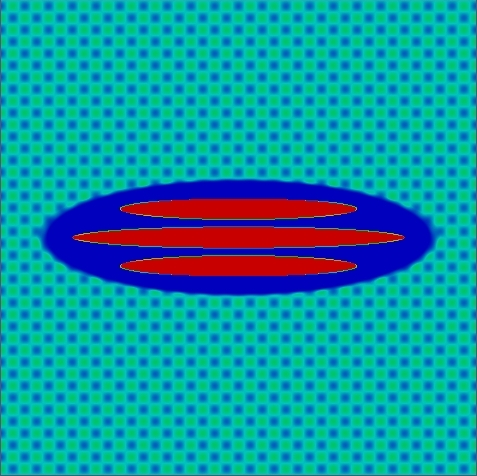
\includegraphics[width=0.41\textwidth]{diffusion_mod_prob_10.jpg}
\end{center}
In the figure we can see a plot of the diffusion coefficient $A^{\epsilon}$. The colorshading is from red (0.05) to blue (0.0005).
The micro structure outside the inner patch is periodic and given by $(8 \pi^2)^{-2} \left( 1 + 2^{-1} \mbox{\rm cos}( 2 \pi \frac{x_0}{\epsilon} ) \mbox{\rm sin}( 2 \pi \frac{x_1}{\epsilon} ) \right)$
with $\epsilon=5 \cdot 10^{-2}$. The transition is smooth. The exact solution is unknown.
\end{modelproblem}
\hrule
\end{document}
